\documentclass[journal]{IEEEtran}
% ---------------------------------------------------------------------------------------------
% Leakage-Free Reproduction and Ensembling of Deep Learning Models for Five-Class
% Diabetic Retinopathy Grading
% Compile: pdflatex main && bibtex main && pdflatex main && pdflatex main   (or upload to Overleaf)
% ---------------------------------------------------------------------------------------------
\usepackage[T1]{fontenc}
\usepackage{cite}
\usepackage{amsmath,amssymb,amsfonts}
\usepackage{graphicx}
\usepackage{booktabs}
\usepackage{multirow}
\usepackage{array}
\usepackage{url}
\usepackage{xcolor}
\usepackage[hidelinks]{hyperref}
\graphicspath{{figures/}}
\newcommand{\figw}{\columnwidth}
\renewcommand{\arraystretch}{1.08}

\begin{document}

\title{Leakage-Free Reproduction and Validation-Selected Ensembling of Deep Learning Models for
Five-Class Diabetic Retinopathy Grading}

\author{Akshai~Krishna~KP,
Mohammed~Azhar~Sait,
Karthik~Krishna~K,
and~Rohit~A%
\thanks{The authors are with the [Department], [Institution], [City, Country]
(e-mail: [corresponding author e-mail]). Individual contributions are listed at the end of the
paper.}%
\thanks{Code, trained weights, split files and all result logs are available in the project
repository (DR\_Detection).}}

\markboth{Preprint, November~2026}%
{Akshai Krishna KP \MakeLowercase{\textit{et al.}}: Leakage-Free Reproduction and Ensembling for DR Grading}

\maketitle

% =============================================================================================
\begin{abstract}
Published accuracies for automated diabetic retinopathy (DR) grading vary widely, partly because
headline figures come from binary or referable-DR tasks, or from protocols that leak information
between training and test data. We reproduce ten deep-learning approaches from a 15-paper survey under
one leakage-free protocol, using four public datasets (APTOS~2019, EyePACS, Messidor-2, IDRiD) with
their original grades and no synthetic data. A correlation-based duplicate audit found identical images
with contradictory grades: 43 pairs in APTOS, and 3 in IDRiD, one crossing its official train/test
split. Splits are grouped by patient, exam or duplicate cluster. All model, ensemble and threshold
choices are made on validation data, with thresholds fitted by repeated cross-fitting, and each test
set is evaluated once. The final model, a four-member ensemble with validation-fitted ordinal
thresholds, attains a quadratic weighted kappa of 0.931 (95\% CI 0.913--0.947) and five-class accuracy
of 0.846 on the held-out APTOS test set ($n=525$). For referable DR it reaches sensitivity 0.961,
specificity 0.919 and AUC 0.984. It does not differ significantly from the best single model (McNemar
$p=0.38$). Externally it reaches kappa 0.819 on IDRiD but under-grades Messidor-2, where
EyePACS-trained models generalise far better (referable sensitivity 0.92 vs.\ 0.45). Two published
claims, of 99\% and 94--97\% accuracy, do not reproduce without leakage. Leakage-free evidence does not
support $\geq$95\% five-class accuracy on these datasets, whereas referable-DR detection approaches
that level.
\end{abstract}

\begin{IEEEkeywords}
Diabetic retinopathy, fundus photography, deep learning, reproducibility, data leakage,
ensemble learning, ordinal regression, external validation.
\end{IEEEkeywords}

% =============================================================================================
\section{Introduction}
\IEEEPARstart{D}{iabetic} retinopathy is a leading cause of preventable vision loss in working-age
adults. Its global burden is projected to keep rising with the prevalence of diabetes~\cite{teo2021global}.
Screening programmes grade colour fundus photographs on the International Clinical DR (ICDR)
scale~\cite{wilkinson2003icdr}: 0~No DR, 1~Mild, 2~Moderate, 3~Severe non-proliferative and
4~Proliferative DR (PDR). Patients with grade~2 or worse are usually \emph{referred} to an
ophthalmologist. Deep convolutional networks have reached specialist-level performance on referable-DR
detection~\cite{gulshan2016development,abramoff2018pivotal}, and a large literature now reports
five-class grading accuracies above 95\%.

Those figures are hard to compare. While surveying 15 recent papers we found that many headline
numbers belong to different tasks:
\begin{itemize}
\item binary DR detection~\cite{butt2022hybrid,zafar2025lightweight};
\item referable DR~\cite{gulshan2016development,papadopoulos2021mil};
\item three-class grouping~\cite{butt2022hybrid};
\item referable diabetic macular edema~\cite{yaqoob2021resnet}.
\end{itemize}
Some come from protocols with \emph{leakage}~\cite{kaufman2012leakage}. One study augments its images
\emph{before} the random train/test split, so augmented copies of training images enter the test
set~\cite{zafar2025lightweight}. Public datasets also contain duplicated photographs, sometimes with
contradictory grades, which inflate scores whenever copies straddle a split. Finally, accuracy alone
is misleading on DR data: 73.5\% of EyePACS images are grade~0, so a constant predictor already
reaches 73.5\%.

This paper is a \emph{reproducibility and benchmarking study}, not a new architecture. It asks a
simple question: \emph{under a single, leakage-free protocol on public data, how
well can the surveyed approaches grade DR into five classes, and how good can a carefully selected
model become?} Our contributions are:
\begin{enumerate}
\item \textbf{Task audit.} An audit of what task each surveyed paper actually solved, verified
against the original texts where available. It shows that no verified study reaches $\geq$95\% on
honest five-class grading.
\item \textbf{Ten reproductions under one protocol.} Each is labelled faithful, adapted or baseline,
and uses only genuine images: no GAN or synthetic data, so one GAN-based component was deliberately
excluded.
\item \textbf{Duplicate audit.} The audit exposes identical images with conflicting grades in APTOS
and IDRiD, including a pair across IDRiD's official train/test split. A transparent exclusion policy
never alters official test sets.
\item \textbf{Validation-only selection.} Ensemble members, decision rule and ordinal thresholds are
chosen from 770 candidates. Repeated cross-fitting prevents threshold fitting from biasing the
choice. The test set is evaluated once afterwards, with bootstrap intervals and paired significance
tests.
\item \textbf{Two external tests.} APTOS$\rightarrow$IDRiD and EyePACS$\rightarrow$Messidor-2 show
that the training distribution, more than the architecture, determines cross-site robustness.
\end{enumerate}

% =============================================================================================
\section{Related Work and Task Audit}
\label{sec:related}
We reviewed 15 papers. Three are reviews~\cite{dejene2025screening,tato2025review,subramanian2022styles},
one studies hand-crafted exudate features~\cite{sisodia2017preprocessing}, one is an early CNN
baseline~\cite{pratt2016cnn}, one is a private-data multi-task system~\cite{dai2021deepdr}, and nine
propose or evaluate deep models. We obtained the full texts of five papers
\cite{butt2022hybrid,gulshan2016development,zafar2025lightweight,yaqoob2021resnet,papadopoulos2021mil}
and the code of one~\cite{abbasi2025adaptive}. The rest are characterised from the survey only.
Table~\ref{tab:audit} summarises what each headline number measures.

\begin{table*}[!t]
\caption{Task Audit of the Surveyed Deep-Learning Papers. ``Verified'' Means the Original Text or
Code Was Read.}
\label{tab:audit}
\centering
\footnotesize
\begin{tabular}{@{}p{3.6cm}p{2.5cm}p{8.4cm}c@{}}
\toprule
Paper (model) & Headline claim & Actual task / protocol & Verified \\
\midrule
Dixit \& Jha~\cite{dixit2025effnet} (EffNet-B3+SE) & 88.44\%, $\kappa$ 0.88 (APTOS) & Multiclass APTOS; class count and protocol not verifiable (paywalled) & -- \\
Butt et al.~\cite{butt2022hybrid} (GoogLeNet + ResNet18 $\rightarrow$ SVM) & 97.8\% / 89.29\% & Binary, and \textbf{3-class} (0 / 1--2 / 3--4) on an undersampled balanced subset; 89.29\% is average class accuracy & yes \\
Gulshan et al.~\cite{gulshan2016development} (Inception-v3) & AUC 0.991 / 0.990 & \textbf{Referable DR}; 128k private multiply-graded images; 10-network ensemble & yes \\
Abbasi et al.~\cite{abbasi2025adaptive} (AGC + CNN) & 95.88\% & Probably binary; includes GAN cataract restoration (excluded here) & code \\
Zafar et al.~\cite{zafar2025lightweight} (two-stage CNN) & 99.06\% / 90.75\% & Binary + 4-class severity; \textbf{augmentation before the random split} (leakage); own leak-free 5-class: 80.08\%, $\kappa$ 0.70 & yes \\
Yaqoob et al.~\cite{yaqoob2021resnet} (ResNet50$\rightarrow$RF) & 96\% / 75.09\% & Messidor-2: referable DME (majority 91.1\%); EyePACS five-class (majority 73.5\%) & yes \\
Papadopoulos et al.~\cite{papadopoulos2021mil} (attention-MIL) & AUC 0.961 / 0.976 & \textbf{Referable DR}; 0.961 from a 5-model ensemble & yes \\
Banerjee et al.~\cite{banerjee2025review} (DenseNet-169, ViT-B/16) & ``highest accuracy'' & Review; no traceable experimental configuration & -- \\
Sushith et al.~\cite{sushith2025hybrid} (MS-CNN+LSTM) & 94--97\%, F1 $>$ 0.99 & Claimed five-class EyePACS; implausible per-class F1 and dataset size & -- \\
\bottomrule
\end{tabular}
\end{table*}

The verified papers therefore measure easier tasks than five-class grading, or report numbers
inflated by leakage or by majority-class prevalence. Leakage-free five-class APTOS results are
typically 80--88\% accuracy, and the reported EyePACS results lie close to the 73.5\% majority
baseline. Reference standards also matter. Krause et~al.~\cite{krause2018grader} showed substantial
grader variability and released adjudicated Messidor-2 grades, which we use as an external reference.

% =============================================================================================
\section{Materials}
\label{sec:materials}

\subsection{Datasets}
We use four public datasets with their original labels (Table~\ref{tab:data}):
\begin{itemize}
\item \textbf{APTOS~2019}~\cite{aptos2019}: the labelled training set; its test labels are private.
\item \textbf{EyePACS}~\cite{eyepacs2015}: the official Kaggle training archive, 35{,}126 images of
17{,}563 patients.
\item \textbf{Messidor-2}~\cite{decenciere2014messidor,abramoff2013messidor2}, with the adjudicated
grades of~\cite{krause2018grader}; 4 ungradable images are excluded.
\item \textbf{IDRiD} disease grading~\cite{porwal2018idrid}.
\end{itemize}
No synthetic, GAN-generated or pseudo-labelled data are used anywhere.

\begin{table}[!t]
\caption{Datasets After the Duplicate Policy and Their Use}
\label{tab:data}
\centering
\footnotesize
\setlength{\tabcolsep}{3pt}
\resizebox{\columnwidth}{!}{%
\begin{tabular}{@{}lrrrrrrl@{}}
\toprule
Dataset & $N$ & 0 & 1 & 2 & 3 & 4 & Use \\
\midrule
APTOS & 3{,}486 & \multicolumn{5}{c}{(of 3{,}662: 1805/370/999/193/295)} & train/val/test \\
EyePACS & 35{,}126 & 25{,}810 & 2{,}443 & 5{,}292 & 873 & 708 & pretraining \\
Messidor-2 & 1{,}740 & 1{,}017 & 268 & 345 & 75 & 35 & external \\
IDRiD & 508 & 167 & 23 & 165 & 92 & 61 & external \\
\bottomrule
\end{tabular}}
\end{table}


\begin{figure*}[!t]
\centering
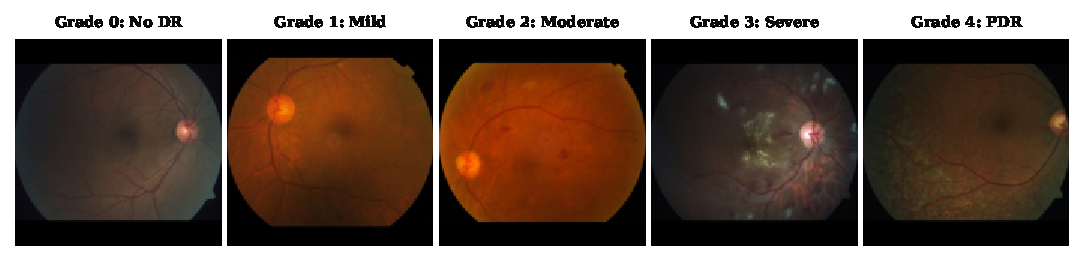
\includegraphics[width=0.95\textwidth]{fig_grades}
\caption{Example APTOS fundus photographs for the five ICDR grades (training split, after retina cropping to 512\,px). Grades are distinguished by microaneurysms (Mild), haemorrhages and hard exudates (Moderate, Severe) and neovascularisation or vitreous haemorrhage (PDR).}
\label{fig:grades}
\end{figure*}

\begin{figure}[!t]
\centering
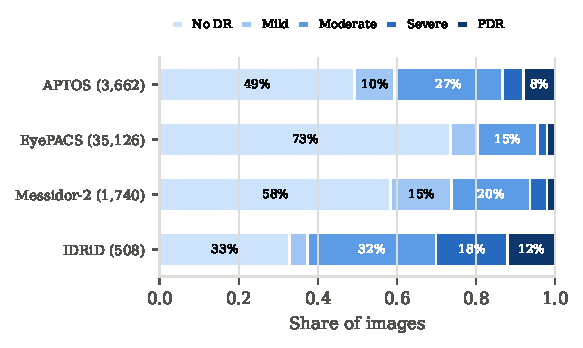
\includegraphics[width=\columnwidth]{fig_class_dist}
\caption{Grade distribution of the four datasets. All are imbalanced; Mild and Severe are minority classes everywhere, and 73\% of EyePACS images are grade~0.}
\label{fig:classdist}
\end{figure}

Fig.~\ref{fig:grades} shows one example per grade and Fig.~\ref{fig:classdist} the class
imbalance of every dataset.

\subsection{Duplicate Audit}
\label{sec:dups}
Duplicates cause leakage when copies straddle splits, and copies with different grades have no
consistent ground truth.

\textbf{Method.} For each image $I$ we compute a 96$\times$96 green-channel high-pass map
$h(I)=G(I)-G_\sigma(I)$, the green channel minus its Gaussian blur, which keeps vessel and lesion
structure. We keep only the central 80\% of the disc radius and standardise the result to zero mean
and unit variance. Pairs whose Pearson correlation is $\geq 0.99$ are linked on the GPU, and linked
pairs are merged into clusters with union-find.

\textbf{Calibration.} Genuine copies score 1.000. With the final interior-only measure, the most
similar \emph{distinct} images score at most 0.873 (APTOS), 0.875 (Messidor-2), 0.770 (IDRiD) and
0.988 (EyePACS, two near-featureless images). The threshold of 0.99 therefore separates copies from
distinct eyes in every dataset (Fig.~\ref{fig:dupcorr}).

\textbf{Rejected variants.} Two simpler designs failed:
\begin{itemize}
\item 64-bit perceptual hashes flagged 181 of 516 IDRiD images, because fundus images are
indistinguishable at 8$\times$8;
\item using the full square chained 16 distinct EyePACS eyes into one cluster, because the camera's
rim notch dominated the correlation.
\end{itemize}

\textbf{Findings} (Fig.~\ref{fig:dups}):
\begin{itemize}
\item \textbf{IDRiD} has six byte-identical pairs. Three carry different grades, including training
image 118 (grade~0) $=$ test image~64 (grade~3), which crosses the official split.
\item \textbf{APTOS} has 148 duplicate pairs (corr.\ $\geq 0.998$; 270 images). Forty-three disagree
on grade: 33 by one grade, 9 by two and 1 by three. Duplicates in APTOS have been discussed informally
by competition participants; here they are quantified and handled under an explicit policy.
\item \textbf{Messidor-2} has four pairs listed under different exams.
\item \textbf{EyePACS} has none.
\end{itemize}

\textbf{Policy}, fixed before any training:
\begin{enumerate}
\item official test sets are never modified; the \emph{training} copy is removed instead;
\item copies with contradictory grades are excluded (79 APTOS, 4 IDRiD images), and the counts are
reported;
\item same-label copies are reduced to one;
\item all copies share one leakage group.
\end{enumerate}
No image was removed for being difficult.
\begin{figure}[!t]
\centering
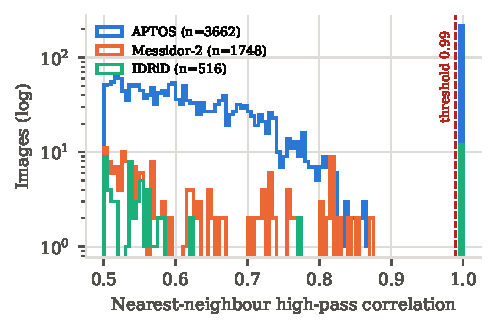
\includegraphics[width=\columnwidth]{fig_dup_corr}
\caption{Distribution of each image's nearest-neighbour high-pass correlation (retina interior, log scale; values below 0.5 omitted). Copies form an isolated spike at 1.0 (APTOS 270, IDRiD 12, Messidor-2 8 images), well separated from distinct images ($\leq$0.875) by the 0.99 threshold.}
\label{fig:dupcorr}
\end{figure}


\begin{figure}[!t]
\centering
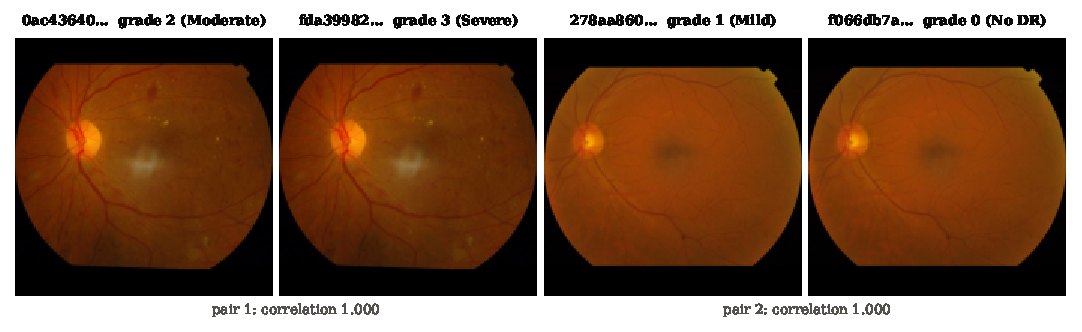
\includegraphics[width=\figw]{fig_duplicates}
\caption{Two of the 43 APTOS duplicate pairs with contradictory grades (correlation 1.000). The
images are pixel-identical after caching but carry different grades (2 vs.~3; 1 vs.~0).}
\label{fig:dups}
\end{figure}

\subsection{Splits}
Each dataset is divided 70/15/15 into train, validation and test with
\texttt{StratifiedGroupKFold} (20 folds, assigned 14/3/3, seed 42). The split is stratified by grade
and grouped by patient (EyePACS, both eyes together), exam (Messidor-2) or duplicate cluster (APTOS,
which has no patient identifiers). An assertion verifies that no group crosses a split. The resulting
sizes are:
\begin{itemize}
\item APTOS: 2{,}437 / 524 / 525, with a test set of 270/51/138/24/42 images per grade;
\item EyePACS: 24{,}586 / 5{,}268 / 5{,}272.
\end{itemize}
Messidor-2 and IDRiD are used in full as external test sets and never for training or tuning.

% =============================================================================================
\section{Methods}
\label{sec:methods}

Fig.~\ref{fig:pipeline} gives an overview of the study.

\begin{figure*}[!t]
\centering
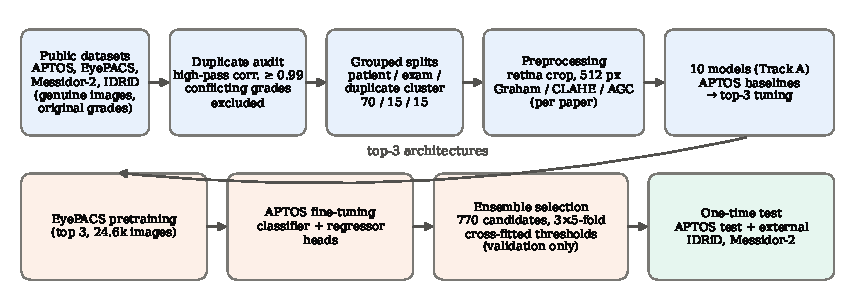
\includegraphics[width=0.92\textwidth]{fig_pipeline}
\caption{Study pipeline. All selection steps use validation data only; each test set is evaluated
once, after the final model is frozen.}
\label{fig:pipeline}
\end{figure*}

\subsection{Preprocessing}
\textbf{Geometric normalisation.} Every photograph is cropped to the retina's bounding box (intensity
threshold plus a morphological opening), padded to a square so the disc is not distorted, resized to
512\,px and cached as JPEG at quality 95 with 4:4:4 chroma.

\textbf{Per-model enhancement.} One enhancement from the surveyed literature is applied on the fly,
per model:
\begin{itemize}
\item \textbf{Graham local-colour subtraction}~\cite{graham2015kaggle}:
$I' = 4I - 4G_{\sigma}(I) + 128$ with $\sigma=\text{size}/30$, used for
EfficientNet~\cite{dixit2025effnet};
\item the same followed by \textbf{zeroing the outer 5\% of the disc}, for
MIL~\cite{papadopoulos2021mil};
\item \textbf{CLAHE} on the LAB lightness channel~\cite{sushith2025hybrid};
\item the \textbf{adaptive gamma correction} of~\cite{abbasi2025adaptive}, ported from the authors'
code: $\gamma(l)=(1-\mathrm{cdf}_m(l))/0.7$ with a histogram mixed 0.4/0.6 with uniform, followed by
V-channel histogram equalisation.
\end{itemize}
The authors' equalisation routine implements the \emph{inverse} mapping. We implement the
equalisation as described in the paper and document the discrepancy.


\begin{figure*}[!t]
\centering
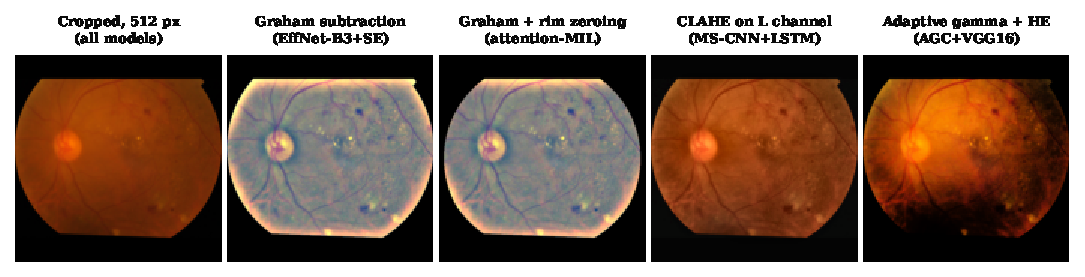
\includegraphics[width=0.95\textwidth]{fig_preproc}
\caption{The preprocessing variants on one APTOS image (Moderate DR): geometric normalisation used by all models, and the per-paper enhancements applied on the fly.}
\label{fig:preproc}
\end{figure*}

Fig.~\ref{fig:preproc} shows all variants on one image.

\textbf{Augmentation.} Random flips, $\pm180^\circ$ rotation, $\pm10$\% scale, 3\% translation and
$\pm0.15$ brightness/contrast, applied only to training images and only after splitting.

\subsection{Models}
Table~\ref{tab:models} lists the ten approaches. Each is labelled:
\begin{itemize}
\item \emph{faithful (F)}: architecture and protocol follow the verified paper;
\item \emph{adapted (A)}: missing details are filled with documented choices;
\item \emph{baseline (B)}: our own configuration of an architecture cited in the survey.
\end{itemize}
ImageNet~\cite{russakovsky2015imagenet} weights come from timm~\cite{wightman2019timm} or
torchvision. The architectures are EfficientNet~\cite{tan2019efficientnet} with an additional
squeeze-and-excitation block~\cite{hu2018se}, Inception-v3~\cite{szegedy2016inception},
DenseNet~\cite{huang2017densenet}, ResNet~\cite{he2016resnet}, GoogLeNet~\cite{szegedy2015googlenet},
VGG~\cite{simonyan2015vgg} and ViT~\cite{dosovitskiy2021vit}. The classical classifiers are random
forests~\cite{breiman2001rf} and SVMs~\cite{cortes1995svm}.

\textbf{Attention-MIL}~\cite{ilse2018attention,papadopoulos2021mil} encodes $K=50$ random
64$\times$64 patches (each $\geq$50\% retina; at test time a grid with 0.75 overlap) into embeddings
$\mathbf{h}_k \in \mathbb{R}^{128}$. It pools them with
$a_k=\mathrm{softmax}_k(\mathbf{w}^\top\tanh(\mathbf{V}\mathbf{h}_k))$ and
$\mathbf{z}=\sum_k a_k\mathbf{h}_k$.

\textbf{The CNN-LSTM}~\cite{sushith2025hybrid} reads the final $7\times7$ multi-scale feature map in
raster order as a 49-step sequence for two LSTM layers~\cite{hochreiter1997lstm} (256 and 128 units),
followed by softmax attention. The paper does not specify this mapping, so it is our assumption.

\textbf{The two-stage CNN}~\cite{zafar2025lightweight} first separates DR from no DR. A second head,
trained on the frozen body, then grades severity among the four DR classes. With stage-one
probabilities $p_1$ and stage-two probabilities $p_2$, the five-class probabilities are
$P(0)=p_1(0)$ and $P(k)=p_1(1)\,p_2(k-1)$ for $k=1,\dots,4$.

Fig.~\ref{fig:arch} details the two custom architectures and the final ensemble.

\begin{figure*}[!t]
\centering
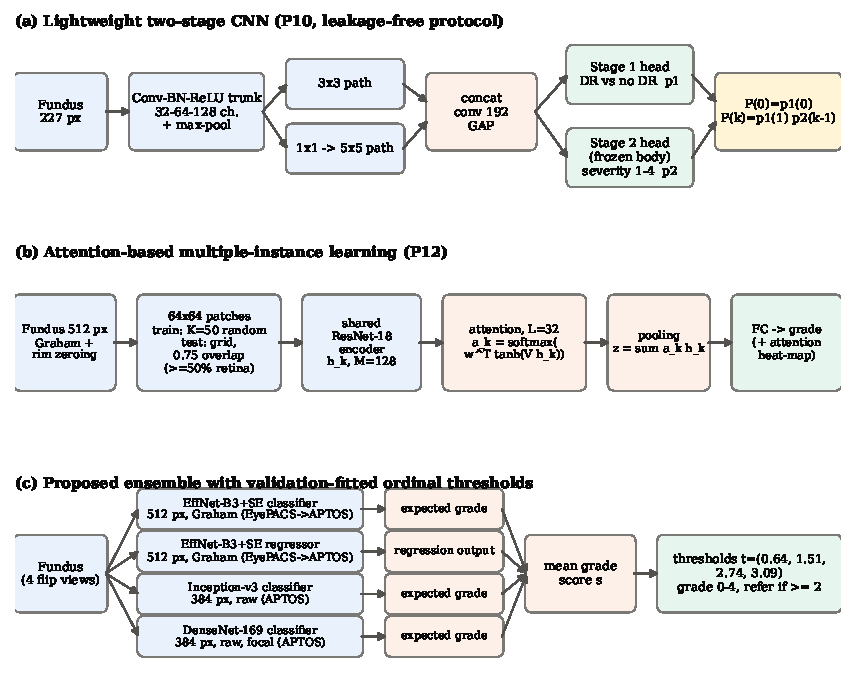
\includegraphics[width=0.9\textwidth]{fig_arch}
\caption{(a) Lightweight two-stage CNN after~\cite{zafar2025lightweight}, trained with a leakage-free protocol. (b) Attention-based MIL after~\cite{papadopoulos2021mil}. (c) The proposed ensemble: four members, four flip views each, averaged grade score cut at validation-fitted ordinal thresholds.}
\label{fig:arch}
\end{figure*}

\begin{table}[!t]
\caption{The Ten Reproduced Approaches (F: Faithful, A: Adapted, B: Baseline)}
\label{tab:models}
\centering
\footnotesize
\setlength{\tabcolsep}{2.5pt}
\resizebox{\columnwidth}{!}{%
\begin{tabular}{@{}llccl@{}}
\toprule
Model & Src. & Px & Params & Notes \\
\midrule
EffNet-B3 + SE & \cite{dixit2025effnet} & 384 & 11.0M & A; SE $r{=}16$, dropout 0.5, Graham \\
Inception-v3 & \cite{gulshan2016development} & 384 & 21.8M & A; public data, 5-class head \\
DenseNet-169 & \cite{banerjee2025review} & 384 & 12.5M & B \\
ResNet-50 (+RF) & \cite{yaqoob2021resnet} & 384 & 23.5M & F; 20-ep.\ fine-tune; RF entropy \\
GoogLeNet+R18$\rightarrow$SVM & \cite{butt2022hybrid} & 224 & 18.3M & F pipeline; 2000-d frozen \\
Two-stage CNN & \cite{zafar2025lightweight} & 227 & 1.6M & A; leak-free protocol \\
Attention-MIL & \cite{papadopoulos2021mil} & 512 & 11.2M & F hyperparameters \\
AGC + VGG16-BN & \cite{abbasi2025adaptive} & 384 & 134.3M & A; GAN step excluded \\
MS-CNN + LSTM & \cite{sushith2025hybrid} & 224 & 1.9M & A; CLAHE, raster sequence \\
ViT-B/16 & \cite{banerjee2025review} & 224 & 85.8M & B \\
\bottomrule
\end{tabular}}
\end{table}

\subsection{Training}
\textbf{Imbalance.} The default loss is class-weighted cross-entropy with
\begin{equation}
w_k = \frac{(N/n_k)^{1/2}}{\frac{1}{C}\sum_j (N/n_j)^{1/2}},
\end{equation}
where $n_k$ is the number of training images of grade $k$, $N$ the total and $C$ the number of
classes. The alternatives are focal loss~\cite{lin2017focal},
$\mathcal{L}_{\mathrm{FL}}=-w_y(1-p_y)^{\gamma}\log p_y$ with $\gamma=2$, and square-root
class-balanced sampling.

\textbf{Optimisation.} Optimisers follow each paper: AdamW~\cite{loshchilov2019adamw},
Adam~\cite{kingma2015adam} or SGD with momentum. Training uses mixed precision, gradient clipping at
5, a cosine schedule with optional warm-up, and early stopping.

\textbf{Model selection.} The best-validation checkpoint maximises
\begin{equation}
S = \tfrac{1}{2}\left(\kappa_w + \mathrm{F1}_{\mathrm{macro}}\right),
\label{eq:score}
\end{equation}
where the quadratic weighted kappa~\cite{cohen1968kappa} is
\begin{equation}
\kappa_w = 1-\frac{\sum_{i,j} W_{ij}O_{ij}}{\sum_{i,j}W_{ij}E_{ij}},\qquad W_{ij}=\frac{(i-j)^2}{(C-1)^2}.
\end{equation}
Here $O$ is the observed confusion matrix and $E$ the matrix expected by chance. $S$ rewards both
ordinal agreement and minority-class performance, unlike accuracy. It was fixed before any experiment.

\textbf{Regression head.} An alternative head predicts a single continuous grade $\hat{g}$ trained
with SmoothL1 loss. For probability-based metrics $\hat{g}$ is mapped to
$p_k\propto\exp(-(\hat{g}-k)^2/(2\cdot0.5^2))$.

\subsection{Transfer from EyePACS}
The three strongest architectures on APTOS validation are pretrained on EyePACS for 12 epochs,
roughly ten times as many updates as APTOS training. They are then fine-tuned on APTOS (learning rate
$10^{-4}$, 15 epochs, one warm-up epoch), each with a classification head and with a regression head.

\subsection{Ensemble and Threshold Selection}
\label{sec:selection}
\textbf{Member outputs.} Each candidate model $m$ outputs class probabilities $\mathbf{p}^{(m)}$ and
a scalar grade score $s^{(m)}$. For a regressor the score is $\hat{g}$; for a classifier it is the
expected grade $\sum_k k\,p^{(m)}_k$. Both are averaged over four flip views (test-time augmentation,
TTA).

\textbf{Candidates.} An ensemble $\mathcal{M}$ (1 to 4 members) is evaluated under two decision
rules:
\begin{align}
\textsc{argmax}:&\quad \hat{y}=\arg\max_k \tfrac{1}{|\mathcal{M}|}\textstyle\sum_{m\in\mathcal{M}}p^{(m)}_k,\\
\textsc{thr}:&\quad \hat{y}=\textstyle\sum_{j=1}^{4}\mathbf{1}\!\left[\bar{s}>t_j\right],\quad
\bar{s}=\tfrac{1}{|\mathcal{M}|}\sum_{m\in\mathcal{M}}s^{(m)},
\end{align}
with ordered thresholds $t_1<\dots<t_4$ fitted by coordinate search (grid 0.02, three sweeps) to
maximise $S$. Ten candidate models give 385 subsets, so there are 770 candidates.

\textbf{Cross-fitting.} Fitting thresholds and scoring them on the same data is optimistic, so every
\textsc{thr} candidate is scored by \emph{repeated cross-fitting}. Over $R=3$ random stratified
5-fold partitions of the validation set, thresholds are fitted on four folds and applied to the
fifth. The score is
\begin{equation}
\hat{S}_{\mathrm{cf}}=\frac{1}{R}\sum_{r=1}^{R} S\!\left(\mathbf{y},\,\hat{\mathbf{y}}^{\mathrm{oof}}_r\right).
\end{equation}
\textsc{argmax} candidates have no fitted parameters and are scored directly.

\textbf{Freezing.} The highest-scoring candidate is frozen, with its thresholds refitted on all
validation data, \emph{before} the test split is read. Selecting the best of many candidates is still
optimistic~\cite{varma2006bias}, which is why the untouched test set is the reported result.

\subsection{Evaluation}
\textbf{Metrics.} We report accuracy, macro and weighted precision, recall and F1, per-class
specificity, one-vs-rest macro ROC-AUC, $\kappa_w$ and confusion matrices.

\textbf{Screening views.} Two binary views are derived from the five-class output: \emph{any DR}
($\geq$1) and \emph{referable DR} ($\geq$2). Each reports sensitivity, specificity, accuracy and AUC,
with $P(\text{grade}\geq k)$ as the score.

\textbf{Statistics.} Confidence intervals are 2{,}000-sample percentile
bootstraps~\cite{efron1994bootstrap}. Models are compared with paired bootstraps and McNemar's exact
test~\cite{mcnemar1947}.

\textbf{Interpretability.} Grad-CAM~\cite{selvaraju2017gradcam} provides qualitative visual
explanations.

\textbf{Implementation.} All experiments use PyTorch~\cite{paszke2019pytorch} and
scikit-learn~\cite{pedregosa2011sklearn} on one NVIDIA RTX~4060 Laptop GPU (8\,GB), with seed 42.

% =============================================================================================
\section{Results}
\label{sec:results}

\subsection{Leakage-Free Baselines on APTOS}
All ten approaches were first trained on APTOS with paper-derived settings and evaluated on
validation. Their configurations were then frozen and the test set evaluated once
(Table~\ref{tab:baselines}, Fig.~\ref{fig:bars}).

\begin{table*}[!t]
\caption{APTOS Five-Class Results of the Ten Approaches (Paper-Default Settings) and the Proposed
Ensemble. Test Columns Are Single, Final Evaluations with 95\% Bootstrap CIs. Ref.: Referable DR
(Grade $\geq$2).}
\label{tab:baselines}
\centering
\footnotesize
\setlength{\tabcolsep}{3.2pt}
\resizebox{\textwidth}{!}{%
\begin{tabular}{@{}lccc|cccccc|c@{}}
\toprule
& \multicolumn{3}{c|}{Validation} & \multicolumn{6}{c|}{Test ($n=525$)} & IDRiD \\
Model & Acc & mF1 & $\kappa_w$ & Acc [CI] & mF1 [CI] & $\kappa_w$ [CI] & AUC & Ref.\ Sens/Spec & Ref.\ AUC & $\kappa_w$ \\
\midrule
ResNet-50~\cite{yaqoob2021resnet} & .887 & .773 & .937 & \textbf{.861} [.830,.891] & \textbf{.743} [.688,.796] & .911 [.879,.939] & .952 & .887/.956 & .984 & .746 \\
ResNet-50+RF~\cite{yaqoob2021resnet} & .876 & .745 & .916 & .844 [.813,.874] & .671 [.611,.726] & .902 [.870,.928] & .949 & .946/.928 & .983 & -- \\
DenseNet-169 & .876 & .764 & .933 & .836 [.804,.867] & .654 [.598,.712] & .904 [.877,.928] & .944 & .902/.944 & .982 & .744 \\
Inception-v3~\cite{gulshan2016development} & .870 & .732 & .917 & .829 [.796,.861] & .687 [.633,.739] & .898 [.872,.922] & .942 & .926/.925 & .977 & .790 \\
EffNet-B3+SE~\cite{dixit2025effnet} & .861 & .737 & .926 & .821 [.789,.853] & .675 [.619,.726] & .903 [.877,.926] & .950 & .936/.919 & .982 & .748 \\
GoogLeNet+R18+SVM~\cite{butt2022hybrid} & .824 & .593 & .864 & .819 [.785,.851] & .594 [.531,.651] & .850 [.812,.883] & .922 & .912/.941 & .972 & -- \\
AGC+VGG16~\cite{abbasi2025adaptive} & .853 & .714 & .916 & .815 [.779,.848] & .646 [.587,.702] & .886 [.857,.913] & .933 & .912/.916 & .974 & .769 \\
Attention-MIL~\cite{papadopoulos2021mil} & .855 & .695 & .890 & .815 [.781,.848] & .631 [.567,.689] & .874 [.841,.903] & .940 & .848/.950 & .980 & .688 \\
ViT-B/16 & .855 & .727 & .910 & .813 [.779,.846] & .625 [.566,.683] & .894 [.867,.918] & .907 & .936/.919 & .974 & .640 \\
Two-stage CNN~\cite{zafar2025lightweight} & .773 & .422 & .754 & .750 [.714,.785] & .398 [.370,.425] & .733 [.688,.776] & .868 & .779/.925 & .949 & .482 \\
MS-CNN+LSTM~\cite{sushith2025hybrid} & .767 & .450 & .820 & .741 [.701,.777] & .405 [.360,.450] & .788 [.755,.819] & .881 & .882/.882 & .957 & .512 \\
\midrule
\textbf{Proposed ensemble} & .903$^\dagger$ & .802$^\dagger$ & .953$^\dagger$ & .846 [.815,.874] & .683 [.626,.734] & \textbf{.931} [.913,.947] & \textbf{.960} & \textbf{.961}/.919 & \textbf{.984} & \textbf{.819} \\
\bottomrule
\multicolumn{11}{l}{\scriptsize $^\dagger$Repeated cross-fitted validation estimate. Majority-class test accuracy: 0.514. IDRiD: all 508 images, external.}
\end{tabular}}
\end{table*}

\begin{figure*}[!t]
\centering
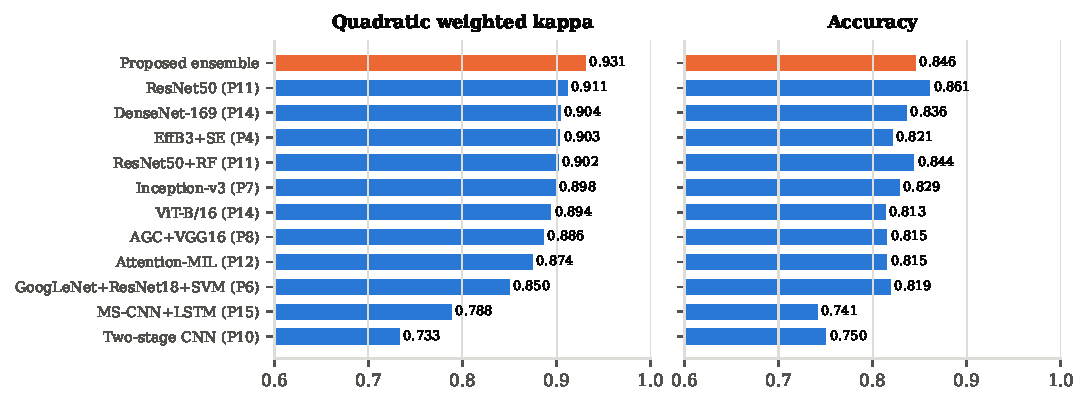
\includegraphics[width=0.85\textwidth]{fig_test_bars}
\caption{APTOS test QWK and accuracy of the ten reproduced approaches and the proposed ensemble
(single final evaluation).}
\label{fig:bars}
\end{figure*}


\begin{figure*}[!t]
\centering
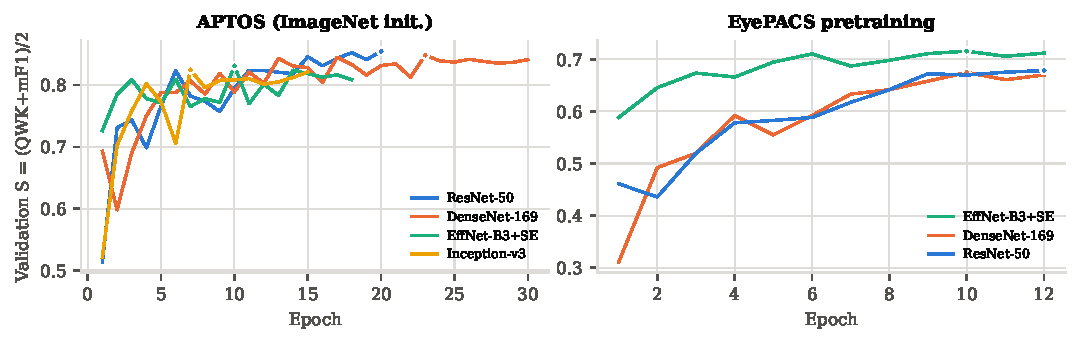
\includegraphics[width=0.9\textwidth]{fig_training}
\caption{Validation selection score $S$ per epoch. Left: APTOS training of the four strongest architectures (ImageNet initialisation). Right: EyePACS pretraining of the top three. Dots mark the selected (best-validation) epochs.}
\label{fig:training}
\end{figure*}

Fig.~\ref{fig:training} shows the validation trajectories of the strongest models.

\textbf{Pretrained CNNs dominate.} Nine models overlap within their confidence intervals (test
accuracy 0.813--0.861, $\kappa_w$ 0.850--0.911): the ImageNet-pretrained CNNs, ViT-B/16, MIL and the
SVM pipeline. The two-stage CNN and the CNN-LSTM are significantly weaker: their CIs do not overlap
those of the top models on $\kappa_w$ or macro-F1.

\textbf{Two-stage CNN.} Without leakage, its first stage separates DR from no DR well (validation
accuracy 0.975, AUC 0.998). Its frozen-body severity stage, however, fails on Severe and PDR (recall
0 on validation).

\textbf{Classical classifiers.} Replacing the network's softmax head with a random forest or SVM never
improved the selection score. On EyePACS validation the RF reached accuracy 0.841 against a majority
baseline of 0.735; its score was 0.664 against 0.678 for its own CNN.

\textbf{Referable DR is much easier than grading.} Referable-DR AUC is 0.95--0.98 for every model,
whereas five-class macro-F1 ranges from 0.40 to 0.74.

\subsection{Reproducibility of the Published Claims}
Table~\ref{tab:claims} compares our results with the original claims.

\textbf{Reproduced or exceeded.} The EfficientNet result~\cite{dixit2025effnet} is close to its
claim. The ResNet+RF EyePACS claim~\cite{yaqoob2021resnet} is matched and exceeded.

\textbf{Not reproducible without leakage.} The two-stage CNN's 99.06\%/90.75\% and the CNN-LSTM's
94--97\% are not reproducible. Our leak-free two-stage result is close to, though below, that paper's
own leak-free figure (80.08\%, $\kappa$ 0.70).

\textbf{Not directly comparable.} The referable-DR papers~\cite{gulshan2016development,papadopoulos2021mil}
used different data and binary training. Our five-class models nevertheless reach referable AUCs of
0.977--0.980 on APTOS.

\begin{table}[!t]
\caption{Published Claims vs.\ Leakage-Free Reproduction (APTOS Test Unless Noted)}
\label{tab:claims}
\centering
\footnotesize
\setlength{\tabcolsep}{2.5pt}
\resizebox{\columnwidth}{!}{%
\begin{tabular}{@{}p{1.9cm}p{2.0cm}p{2.3cm}p{1.9cm}@{}}
\toprule
Approach & Claim & Ours & Verdict \\
\midrule
EffNet-B3+SE & 88.44\%, $\kappa$.88 & 82.1\%, $\kappa_w$.903 & close \\
ResNet50+RF & 75.09\% EyePACS & 84.1\% (EyePACS val) & exceeded \\
Two-stage CNN & 99.06\% bin., 90.75\% 4-cl. & 97.5\% bin.\ (val); 75.0\% 5-cl. & leakage-dependent \\
MS-CNN+LSTM & 94--97\% & 74.1\%, $\kappa_w$.788 & not reproduced \\
Inception-v3 & AUC .991 (rDR) & rDR AUC .977 & different data \\
Attention-MIL & AUC .961 (rDR) & rDR AUC .980 & different task \\
AGC+CNN & 95.88\% (binary?) & 81.5\%, $\kappa_w$.886 & different task \\
\bottomrule
\end{tabular}}
\end{table}

\subsection{Ablation of Training Factors}
The top three models were tuned on validation by changing one factor at a time
(Table~\ref{tab:ablation}). To measure run-to-run noise we re-ran the ResNet-50 baseline with two more
seeds. It scored $S=0.855$, 0.850 and 0.850, a noise level of about $\pm0.005$.

\textbf{Above noise.} Only the 512-pixel input for EfficientNet clearly exceeds the noise ($+0.013$).

\textbf{Preprocessing.} Swapping to the other preprocessing hurt every model: Graham subtraction for
ResNet and DenseNet, raw images for EfficientNet.

\textbf{Rebalancing.} Focal loss and balanced sampling trade overall score for rare-class recall. For
DenseNet, focal loss raises Mild recall from 0.61 to 0.82, and balanced sampling raises Severe recall
from 0.64 to 0.76.


\begin{figure}[!t]
\centering
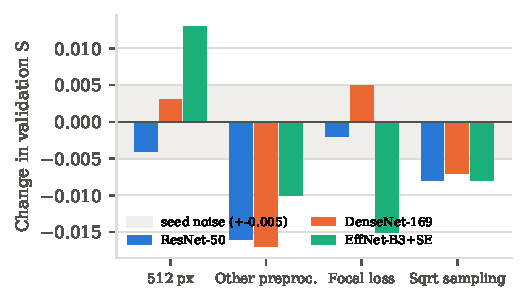
\includegraphics[width=\columnwidth]{fig_ablation}
\caption{One-factor ablation on APTOS validation for the top three architectures. The grey band is the measured seed noise ($\pm$0.005); only 512\,px input for EfficientNet-B3+SE clearly exceeds it.}
\label{fig:ablation}
\end{figure}

\textbf{Schedule length.} A 40-epoch schedule for ResNet-50, whose best epoch had been its last, gave
no gain.

\begin{table}[!t]
\caption{One-Factor Ablation on APTOS Validation: Change in $S$ (Eq.~\ref{eq:score}). Seed Noise
$\approx\pm$0.005.}
\label{tab:ablation}
\centering
\footnotesize
\begin{tabular}{@{}lccc@{}}
\toprule
Factor & ResNet-50 & DenseNet-169 & EffNet-B3+SE \\
\midrule
Baseline $S$ & 0.855 & 0.849 & 0.831 \\
512 px input & $-$0.004 & $+$0.003 & $\mathbf{+0.013}$ \\
Other preprocessing & $-$0.016 & $-$0.017 & $-$0.010 \\
Focal loss ($\gamma$=2) & $-$0.002 & $+$0.005 & $-$0.015 \\
$\sqrt{\cdot}$ balanced sampling & $-$0.008 & $-$0.007 & $-$0.008 \\
40 epochs & 0.000 & -- & -- \\
Focal + 512 px & -- & $+$0.001 & -- \\
\bottomrule
\end{tabular}
\end{table}

\subsection{EyePACS Pretraining and Head Type}
\textbf{EyePACS validation.} EfficientNet-B3+SE at 512\,px reached $\kappa_w=0.815$ and AUC 0.911.
DenseNet-169 (focal loss) and ResNet-50 reached 0.770 and 0.772. Mild DR, often only a few
microaneurysms, was the hardest class (recall 0.17--0.38).

\textbf{After fine-tuning on APTOS} (validation):
\begin{itemize}
\item the regression heads reached the highest $\kappa_w$: 0.938 for DenseNet and 0.933 for
EfficientNet;
\item the classifier heads reached higher accuracy and macro-F1;
\item no single fine-tuned model beat the best APTOS-only model on $S$.
\end{itemize}
Regression and classification heads thus make complementary errors. A regressor errs mostly by one
grade, which $\kappa_w$ rewards; a classifier gets more grades exactly right.

\subsection{The Selected Ensemble}
Repeated cross-fitting selected a four-member \textsc{thr} ensemble ($\hat{S}_{\mathrm{cf}}=0.8776$)
with thresholds $\mathbf{t}=(0.64, 1.51, 2.74, 3.09)$. Its members are the EyePACS-pretrained
EfficientNet-B3+SE classifier and regressor (512\,px, Graham), Inception-v3 (384\,px, raw) and
DenseNet-169 with focal loss (384\,px, raw). The top three candidates differed by less than 0.0011,
so the choice among them is practically a tie. Fig.~\ref{fig:selection} shows the distribution of all
770 candidate scores, and Fig.~\ref{fig:scores} the ensemble's grade scores with the fitted thresholds.

\begin{figure}[!t]
\centering
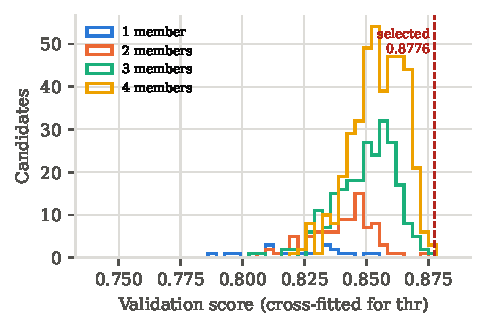
\includegraphics[width=\columnwidth]{fig_selection}
\caption{Validation scores of the 770 candidate ensembles by size (\textsc{thr} candidates cross-fitted). Larger ensembles score higher on average; the selected candidate is marked.}
\label{fig:selection}
\end{figure}

\begin{figure*}[!t]
\centering
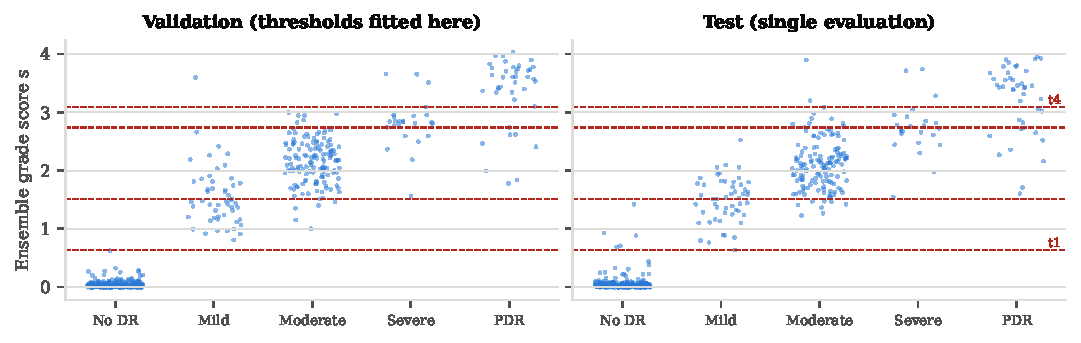
\includegraphics[width=0.9\textwidth]{fig_scores}
\caption{Ensemble grade score $\bar{s}$ per image grouped by true grade, on validation (where the thresholds, dashed, were fitted) and on the test set (single evaluation). Mild and Severe overlap their neighbours, which explains their lower recall.}
\label{fig:scores}
\end{figure*}


\textbf{Test results.} On the APTOS test set (Table~\ref{tab:baselines}, Fig.~\ref{fig:cm}) the
ensemble attains:
\begin{itemize}
\item $\kappa_w=0.931$ [0.913, 0.947], the highest of all 19 single models evaluated on the test set
(best single model 0.926);
\item five-class AUC 0.960, accuracy 0.846 and macro-F1 0.683;
\item weighted F1 0.842.
\end{itemize}
The validation-to-test drop ($-0.057$ accuracy, $-0.022$ $\kappa_w$) reflects the optimism of picking
the maximum of 770 candidates on 524 images~\cite{varma2006bias}.

\textbf{Per-class behaviour.}
\begin{itemize}
\item Per-class recall is 0.981 (No DR), 0.471 (Mild), 0.862 (Moderate), 0.333 (Severe) and 0.667
(PDR).
\item Of the 81 errors, 69 are one grade off and 12 two grades off (10 PDR$\rightarrow$Moderate,
2 Moderate$\rightarrow$PDR). None are further, which explains the high $\kappa_w$ despite moderate
accuracy.
\item The weak classes sit at the Mild/Moderate and Severe/Moderate boundaries, where APTOS itself
contains contradictory duplicate grades (Section~\ref{sec:dups}).
\end{itemize}


\begin{figure*}[!t]
\centering
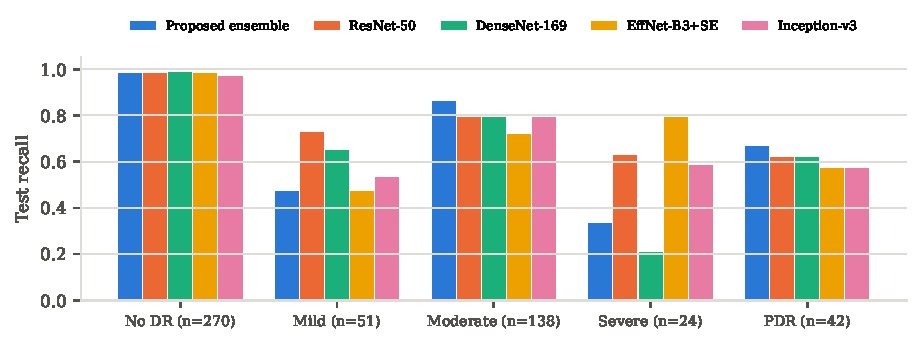
\includegraphics[width=0.95\textwidth]{fig_perclass}
\caption{Per-class test recall of the proposed ensemble and the four strongest single models (APTOS test, $n$ per class in brackets). The ensemble has the highest Moderate recall; Severe recall varies most between models (0.21--0.79), as expected with only 24 Severe test images.}
\label{fig:perclass}
\end{figure*}

Fig.~\ref{fig:perclass} compares per-class recall with the strongest single models.

\textbf{Screening performance.}
\begin{itemize}
\item \textbf{Referable DR:} sensitivity 0.961 [0.932, 0.985], specificity 0.919 [0.889, 0.948],
accuracy 0.935 [0.914, 0.956] and AUC 0.984 [0.976, 0.992]. All eight missed referable eyes were
graded Mild, none No DR.
\item \textbf{Any DR:} sensitivity 0.996, specificity 0.982 and AUC 0.9997.
\end{itemize}

\begin{figure}[!t]
\centering
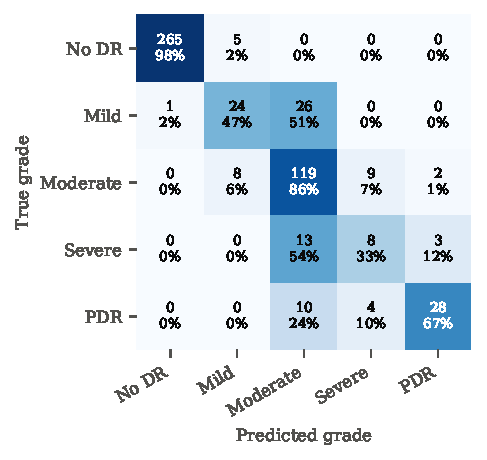
\includegraphics[width=0.92\columnwidth]{fig_confusion_test}
\caption{Confusion matrix of the proposed ensemble on the APTOS test set ($n=525$; counts and
row-normalised percentages). All errors are within two grades, and 69 of the 81 errors are one grade
off.}
\label{fig:cm}
\end{figure}

\textbf{Comparison with the best single model} (ResNet-50, paired bootstrap):
\begin{itemize}
\item $\Delta\kappa_w=+0.019$ [$-0.001$, $+0.046$], with $P(\Delta>0)=0.97$;
\item $\Delta$accuracy $=-0.016$ [$-0.048$, $+0.013$];
\item $\Delta$macro-F1 $=-0.061$ [$-0.124$, $+0.002$].
\end{itemize}
McNemar's test on per-image correctness gives 28 vs.\ 36 discordant images ($p=0.38$). Neither model
is significantly better. The ensemble leads on the ordinal metric and the single CNN on exact
accuracy. We keep the ensemble as the final model because it was selected by the pre-declared
validation rule. Switching after inspecting test results would be selection on the test set.

\subsection{Cross-Dataset Generalisation}
Table~\ref{tab:external} and Fig.~\ref{fig:roc} report the external evaluations. Thresholds are
carried over unchanged.

\textbf{APTOS$\rightarrow$IDRiD.} The ensemble retains the best $\kappa_w$ (0.819) and a referable
AUC of 0.976, but five-class accuracy falls to 0.593. Severe recall is only 0.16, since most IDRiD
Severe images are graded Moderate.

\textbf{Messidor-2.} The APTOS ensemble ranks referable cases well (AUC 0.948) but systematically
under-grades them by about one grade: 187 of 345 Moderate images are called Mild, and 207 of 268 Mild
images are called No DR. Referable sensitivity is therefore only 0.451 at the frozen thresholds.


\begin{figure*}[!t]
\centering
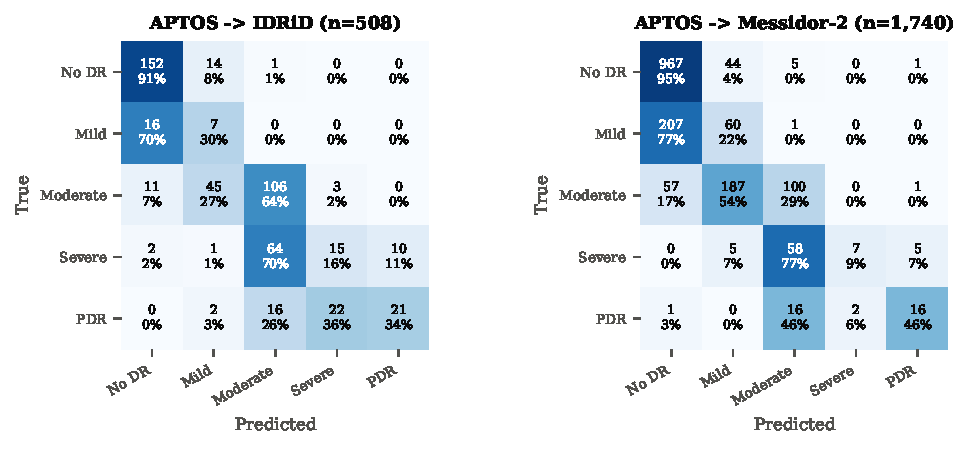
\includegraphics[width=0.9\textwidth]{fig_external_cm}
\caption{Confusion matrices of the proposed ensemble on the external datasets (frozen APTOS thresholds). On Messidor-2 the errors lie mostly one grade below the diagonal, i.e.\ systematic under-grading.}
\label{fig:extcm}
\end{figure*}

Fig.~\ref{fig:extcm} shows the external confusion matrices.

\textbf{EyePACS-trained models generalise better.} On Messidor-2 they achieve higher accuracy
(0.719--0.763), $\kappa_w$ (0.756--0.785) and macro-F1 (0.615--0.651). Their referable sensitivity is
0.87--0.92 at specificity 0.85--0.91; EfficientNet-B3+SE reaches AUC 0.967. The training distribution
(multi-site, 24.6k images) therefore matters more for cross-site robustness than the architecture or
the ensembling.

\begin{table}[!t]
\caption{External Evaluation (All Gradable, Non-Duplicate Images; Never Used for Training or Tuning)}
\label{tab:external}
\centering
\footnotesize
\setlength{\tabcolsep}{2.6pt}
\resizebox{\columnwidth}{!}{%
\begin{tabular}{@{}llcccc@{}}
\toprule
Train$\rightarrow$Test & Model & Acc & $\kappa_w$ & mF1 & Ref.\ Sens/Spec/AUC \\
\midrule
APTOS$\rightarrow$IDRiD & Ensemble & .593 & \textbf{.819} & .462 & .808/.995/\textbf{.976} \\
 & Inception-v3 & .575 & .790 & .445 & .802/.974/.966 \\
 & AGC+VGG16 & \textbf{.596} & .769 & .469 & .818/.963/.966 \\
 & EffNet-B3+SE & .577 & .748 & \textbf{.481} & .874/.826/.942 \\
\midrule
EyePACS$\rightarrow$Mess.-2 & ResNet-50 & \textbf{.763} & .784 & .650 & .884/.907/.963 \\
 & DenseNet-169 & .742 & \textbf{.785} & .615 & .868/.906/.953 \\
 & EffNet-B3+SE & .719 & .756 & \textbf{.651} & \textbf{.923}/.847/\textbf{.967} \\
APTOS$\rightarrow$Mess.-2 & Ensemble & .661 & .725 & .434 & .451/.995/.948 \\
\bottomrule
\end{tabular}}
\end{table}

\begin{figure}[!t]
\centering
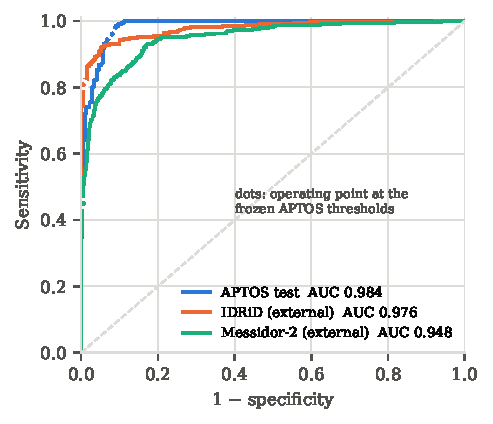
\includegraphics[width=0.92\columnwidth]{fig_roc_referable}
\caption{Referable-DR ROC curves of the proposed ensemble. Dots mark the operating point of the
frozen APTOS thresholds; on Messidor-2 the ranking is good (AUC 0.948) but the operating point is
miscalibrated.}
\label{fig:roc}
\end{figure}

\subsection{Interpretability and Cost}
\textbf{Grad-CAM} (Fig.~\ref{fig:gradcam}) on the EfficientNet classifier member highlights clusters
of exudates and haemorrhages in Moderate and Severe eyes. Maps for Mild eyes are diffuse, consistent
with microaneurysms being only a few pixels wide at 512\,px. In some PDR eyes the map centres on the
optic-disc region. This is plausible for disc neovascularisation, but we cannot exclude a shortcut
without lesion-level validation.

\textbf{Cost.} The ensemble has 56.3M parameters and needs about 174\,ms per image on the laptop GPU
(batch 1, four-flip TTA, including image loading). The best single model, ResNet-50, needs about
4\,ms.

\begin{figure*}[!t]
\centering
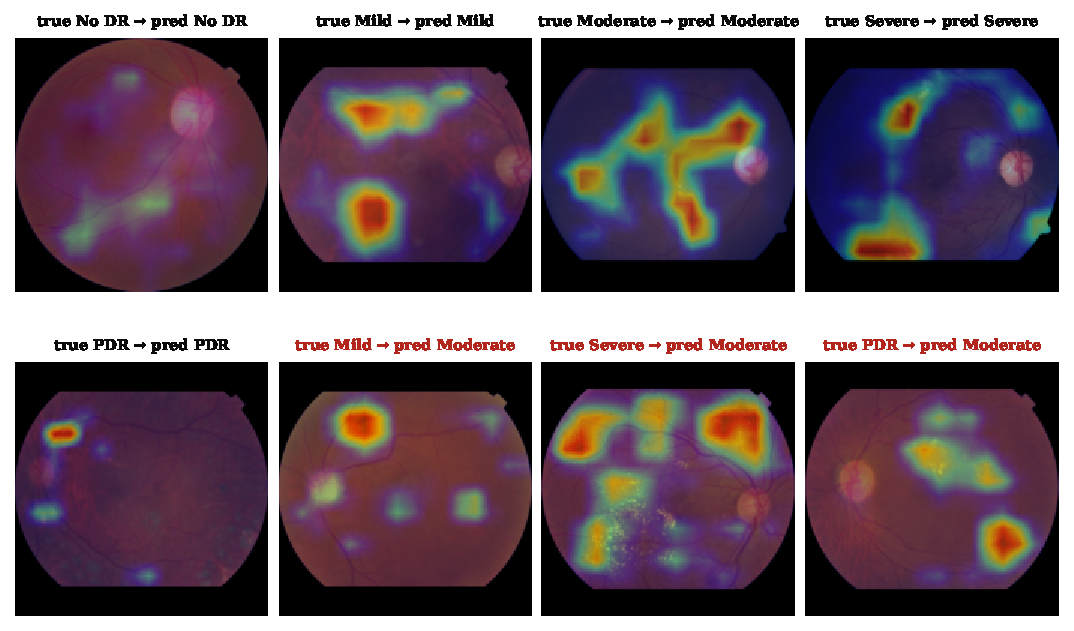
\includegraphics[width=0.82\textwidth]{fig_gradcam}
\caption{Grad-CAM of the EfficientNet-B3+SE (EyePACS$\rightarrow$APTOS) member on APTOS test images.
Top row and bottom-left: correct grades. Red titles: typical one-grade-off errors towards Moderate.}
\label{fig:gradcam}
\end{figure*}

% =============================================================================================
\section{Discussion}
\label{sec:discussion}

\textbf{What performance is attainable?} Under a leakage-free protocol the best five-class result
on APTOS is $\kappa_w\approx0.93$ with accuracy $\approx0.85$. A $\kappa_w$ above 0.81 is ``almost
perfect'' agreement on the conventional scale~\cite{landis1977kappa}, in the range of human
inter-grader agreement~\cite{krause2018grader}.

Accuracies of 95\% or more for five classes, common in the surveyed literature, are not supported by
any verified leakage-free result. The gap has four sources:
\begin{enumerate}
\item task conflation (Table~\ref{tab:audit});
\item leakage through pre-split augmentation;
\item duplicates across splits;
\item intrinsic label noise. In APTOS, 43 pixel-identical pairs carry different grades.
\end{enumerate}
Referable-DR detection, in contrast, reaches 93.5\% accuracy and 0.984 AUC. Its upper confidence
bound (95.6\%) includes the 95\% level.

\textbf{What helps?} In decreasing order of effect:
\begin{enumerate}
\item multi-site pretraining data, for generalisation;
\item ensembling heterogeneous members with ordinal thresholds, for $\kappa_w$ and AUC;
\item higher input resolution for compound-scaled networks;
\item regression heads, for ordinal agreement.
\end{enumerate}
Preprocessing variants, loss rebalancing, longer schedules, P8's adaptive gamma correction and
classical classifiers on deep features gave no reliable gain.

\textbf{Selection hygiene.} Repeated cross-fitting removes the bias of fitting thresholds on the data
used to rank candidates. It cannot remove the winner's-curse bias of choosing among 770
candidates~\cite{varma2006bias}. The 5.7-point validation-to-test drop quantifies that bias and shows
why a single untouched test evaluation is indispensable.

\textbf{Clinical reading.} On APTOS-like images the model would refer 96\% of referable eyes at 92\%
specificity. The eight missed eyes were all graded Mild, never healthy. Across sites, however,
threshold miscalibration (Messidor-2 sensitivity 0.45 despite AUC 0.948) shows that deployment
requires site-specific calibration or multi-site training data. The model is a research artefact, not
a medical device.

% =============================================================================================
\section{Limitations}
\textbf{Scope.}
\begin{itemize}
\item EyePACS training was restricted to the three strongest architectures.
\item Referable-DR results are derived from five-class models rather than dedicated binary training.
\item The original binary and three-class tasks of~\cite{butt2022hybrid} were not re-run.
\end{itemize}

\textbf{Source access.} Four papers could only be characterised from the survey, so their settings
are partly ours.

\textbf{Definitions.} The referable-DR definition excludes macular edema, because the public grade
labels lack it.

\textbf{Statistics.}
\begin{itemize}
\item A single seed was used per configuration, with measured noise of $\pm0.005$ in $S$.
\item The 524-image validation set limits how reliably the selection can rank candidates.
\end{itemize}

\textbf{Explanations.} Grad-CAM evidence is qualitative.

% =============================================================================================
\section{Conclusion}
We reproduced ten DR-grading approaches under one leakage-free protocol on genuine public data. We
audited duplicates and task definitions, and selected an ensemble with cross-fitted ordinal thresholds
using validation data only.

\textbf{Results.} The final model reaches $\kappa_w=0.931$ for five-class grading and a referable-DR
AUC of 0.984, with sensitivity 0.961, on an untouched test set. It ranks first by $\kappa_w$, while not
being significantly different from the best single CNN.

\textbf{Main lessons.}
\begin{itemize}
\item Honest five-class accuracy on these data lies near 85\%, not 95\%.
\item Duplicate and task audits are prerequisites for meaningful comparison.
\item Multi-site training data determine cross-site robustness.
\end{itemize}

\textbf{Future work.}
\begin{itemize}
\item Joint EyePACS+APTOS training of the ensemble members, with per-site calibration.
\item Nested cross-validation for selection.
\item Higher-resolution or lesion-supervised models for Mild DR.
\item Dedicated referable-DR training.
\end{itemize}

% =============================================================================================
\section*{Data and Code Availability}
All datasets are public: APTOS~2019 and EyePACS (Kaggle), Messidor-2 (ADCIS, with the adjudicated
grades of~\cite{krause2018grader}) and IDRiD. The project repository includes:
\begin{itemize}
\item split files, duplicate lists and per-run configurations, histories and predictions;
\item the packaged ensemble with an inference script;
\item a step-by-step replication guide.
\end{itemize}

\section*{Acknowledgment}
The authors thank the creators of APTOS, EyePACS, Messidor-2 and IDRiD for making their data
available. This work builds on a literature survey of 15 papers prepared within the project team.

\bibliographystyle{IEEEtran}
\bibliography{references}

\clearpage
\onecolumn
\section*{Author Contributions}
\addcontentsline{toc}{section}{Author Contributions}
\begin{table}[!h]
\centering
\footnotesize
\setlength{\tabcolsep}{3.5pt}
\renewcommand{\arraystretch}{1.25}
\begin{tabular}{@{}>{\raggedright\arraybackslash}p{3.0cm}>{\raggedright\arraybackslash}p{4.1cm}>{\raggedright\arraybackslash}p{5.0cm}>{\raggedright\arraybackslash}p{5.2cm}@{}}
\toprule
Author (roll no.) & Literature survey & Data science & Machine learning \\
\midrule
\textbf{Akshai Krishna KP} (CS24B1096) &
P2 ML review~\cite{tato2025review}; P6 hybrid features + SVM~\cite{butt2022hybrid};
P10 two-stage CNN~\cite{zafar2025lightweight}; P14 DenseNet/ViT review~\cite{banerjee2025review} &
Data acquisition and validation (APTOS, EyePACS, Messidor-2 licence request, IDRiD); retina-crop
cache; preprocessing library (Graham, rim zeroing, CLAHE, port of the adaptive gamma correction) &
Transfer-learning backbones: EfficientNet-B3+SE, Inception-v3, DenseNet-169, ViT-B/16, and their
APTOS baselines; Grad-CAM interpretability \\
\addlinespace
\textbf{Mohammed Azhar Sait} (CS24B1103) &
P1 systematic review~\cite{dejene2025screening}; P5 exudate features~\cite{sisodia2017preprocessing};
P9 early CNN~\cite{pratt2016cnn}; P13 DeepDR~\cite{dai2021deepdr} &
Duplicate audit: high-pass correlation measure, threshold calibration, union-find clustering and the
exclusion policy (Section~\ref{sec:dups}) &
Training engine (mixed precision, weighted and focal losses, early stopping, regression head);
validation-only ensemble and ordinal-threshold selection with repeated cross-fitting
(Section~\ref{sec:selection}) \\
\addlinespace
\textbf{Karthik Krishna K} (CS24I1009) &
P3 bibliometric review~\cite{subramanian2022styles}; P7 Inception-v3~\cite{gulshan2016development};
P11 ResNet-50 + RF~\cite{yaqoob2021resnet}; P15 MS-CNN+LSTM~\cite{sushith2025hybrid} &
Patient-, exam- and cluster-grouped stratified splits with leakage assertions; class-imbalance
analysis and class weighting; majority-class baselines &
Classical and custom pipelines: ResNet-50 + random forest, GoogLeNet + ResNet-18 + SVM (validation
grid search), lightweight two-stage CNN; one-factor ablations and seed-noise measurement \\
\addlinespace
\textbf{Rohit A} (CS24I1010) &
P4 EfficientNet-B3+SE~\cite{dixit2025effnet}; P8 adaptive enhancement~\cite{abbasi2025adaptive};
P12 attention-MIL~\cite{papadopoulos2021mil}; consolidated task-audit table (Table~\ref{tab:audit}) &
Statistical evaluation: metric suite, bootstrap confidence intervals, McNemar and paired tests;
cross-dataset analysis (APTOS$\rightarrow$IDRiD, EyePACS$\rightarrow$Messidor-2) &
Attention-MIL, AGC + VGG16 and multi-scale CNN-LSTM; EyePACS pretraining and APTOS fine-tuning with
classification and regression heads \\
\bottomrule
\end{tabular}
\end{table}


\end{document}
